\documentclass[a4paper]{article}

\usepackage[margin=1in]{geometry}
\usepackage{amsmath,amsfonts,mathtools,amsthm,amssymb}
\usepackage[l2tabu,orthodox]{nag}
\usepackage{microtype} % fixes spacing or whatever
\usepackage{enumitem}
\usepackage{tikz-cd}
\usepackage{xcolor}
\usepackage{physics}
\usepackage{mathrsfs}
\usepackage{cancel}
% \usepackage{libertine,libertinust1math}
\usepackage{eucal}
\usepackage[toc,page]{appendix}
\usepackage{pgfplots}
\pgfplotsset{compat=1.18}

\newtheorem{proposition}{Proposition}
\newtheorem{theorem}{Theorem}
\newtheorem{lemma}{Lemma}
\newtheorem{corollary}{Corollary}

\theoremstyle{definition}
\newtheorem{remark}{Remark}
\newtheorem{definition}{Definition}
\newtheorem{example}{Example}

% \usepackage[sc,osf]{mathpazo}   % With old-style figures and real smallcaps.
% \linespread{1.025}              % Palatino leads a little more leading
% % Euler for math and numbers
% \usepackage[euler-digits,small]{eulervm}
% \AtBeginDocument{\renewcommand{\hbar}{\hslash}}

\usepackage{etoolbox}
\usepackage{dynkin-diagrams}
\def\row#1/#2!{\dynkin{#1}{#2}\\}
\newcommand{\tble}[1]{
   \renewcommand*\do[1]{\row##1!}
   \[
      \begin{array}{ll}\docsvlist{#1}\end{array}
   \]
}

\allowdisplaybreaks

\renewcommand{\epsilon}{\varepsilon}
% \renewcommand{\phi}{\varphi}

\DeclareMathAlphabet{\mathpzc}{OT1}{pzc}{m}{it}

\newcommand{\goth}[1]{\mathfrak{#1}}
\newcommand{\red}[1]{#1_{\text{red}}}
\newcommand{\ad}[1]{#1_{\text{Ad}}}
\newcommand{\reg}[1]{#1_{\text{reg}}}
\newcommand{\sh}[1]{#1^{\text{sh}}}
\newcommand{\cpdv}[2]{\cfrac{\partial #1}{\partial #2}}

\newcommand{\fA}{\mathcal{A}}
\newcommand{\fB}{\mathcal{B}}
\newcommand{\fC}{\mathcal{C}}
\newcommand{\fD}{\mathcal{D}}
\newcommand{\fE}{\mathcal{E}}
\newcommand{\fF}{\mathcal{F}}
\newcommand{\fG}{\mathcal{G}}
\newcommand{\fH}{\mathcal{H}}
\newcommand{\fI}{\mathcal{I}}
\newcommand{\fJ}{\mathcal{J}}
\newcommand{\fK}{\mathcal{K}}
\newcommand{\fL}{\mathcal{L}}
\newcommand{\fM}{\mathcal{M}}
\newcommand{\fN}{\mathcal{N}}
\newcommand{\fO}{\mathcal{O}}
\newcommand{\fP}{\mathcal{P}}
\newcommand{\fQ}{\mathcal{Q}}
\newcommand{\fR}{\mathcal{R}}
\newcommand{\fS}{\mathcal{S}}
\newcommand{\fT}{\mathcal{T}}
\newcommand{\fX}{\mathcal{X}}
\newcommand{\fY}{\mathcal{Y}}
\newcommand{\fZ}{\mathcal{Z}}

\newcommand{\be}{\mathbf{e}}
\newcommand{\bx}{\mathbf{x}}
\newcommand{\bone}{\mathbf{1}}
\newcommand{\cx}{\bar{x}}
\newcommand{\cy}{\bar{y}}
\newcommand{\vx}{\vec{x}}
\newcommand{\vsigma}{\vec{\sigma}}
\newcommand{\tzeta}{\tilde{\zeta}}

\newcommand{\gm}{\goth{m}}
\newcommand{\gp}{\goth{p}}
\newcommand{\gF}{\goth{F}}
\newcommand{\gU}{\goth{U}}
\newcommand{\gV}{\goth{V}}

\newcommand{\A}{\mathbf{A}}
\newcommand{\C}{\mathbf{C}}
\newcommand{\F}{\mathbf{F}}
\newcommand{\G}{\mathbf{G}}
\newcommand{\bH}{\mathbf{H}}
\newcommand{\N}{\mathbf{N}}
\newcommand{\PP}{\mathbf{P}}
\newcommand{\Q}{\mathbf{Q}}
\newcommand{\R}{\mathbf{R}}
\newcommand{\Z}{\mathbf{Z}}

\newcommand{\dlog}{\dd\log}

\newcommand\srestr[2]{{\left.\kern-\nulldelimiterspace #1\vphantom{\small|} \right|_{#2}}}
\newcommand\restr[2]{{\left.\kern-\nulldelimiterspace #1 \vphantom{\big|} \right|_{#2}}}
\newcommand\gsec[2]{\Gamma({#1}, {#2})}
\newcommand\gsecx[1]{\Gamma(X, {#1})}

\DeclareMathOperator{\chr}{char}
\DeclareMathOperator{\rProj}{\mathbf{Proj}}
\DeclareMathOperator{\rSpec}{\mathbf{Spec}}
\DeclareMathOperator{\rHom}{\mathbf{Hom}}
\DeclareMathOperator{\rExt}{\mathbf{Ext}}
\DeclareMathOperator{\id}{id}
\DeclareMathOperator{\Frac}{Frac}
\DeclareMathOperator{\rk}{rank}
\DeclareMathOperator{\deter}{det}
\DeclareMathOperator{\pic}{Pic}
\DeclareMathOperator{\cacl}{CaCl}
\DeclareMathOperator{\trd}{tr.d.}
\DeclareMathOperator{\cl}{Cl}
\DeclareMathOperator{\depth}{depth}
\DeclareMathOperator{\codim}{codim}
\DeclareMathOperator{\Div}{Div}
\DeclareMathOperator{\coker}{coker}
\DeclareMathOperator{\len}{length}
\DeclareMathOperator{\height}{height}
\DeclareMathOperator{\supp}{Supp}
\DeclareMathOperator{\proj}{Proj}
\DeclareMathOperator{\im}{im}
\DeclareMathOperator{\Hom}{Hom}
\DeclareMathOperator{\Der}{Der}
\DeclareMathOperator{\spec}{Spec}
\DeclareMathOperator{\Aut}{Aut}
\DeclareMathOperator{\ch}{char}
\DeclareMathOperator{\tor}{Tor}
\DeclareMathOperator{\Ann}{Ann}
\DeclareMathOperator{\Syl}{Syl}
\DeclareMathOperator{\Sym}{Sym}
\DeclareMathOperator{\GL}{GL}
\DeclareMathOperator{\SL}{SL}
\DeclareMathOperator{\Stab}{Stab}
\DeclareMathOperator{\Perm}{Perm}
\DeclareMathOperator{\Orb}{Orb}
\DeclareMathOperator{\Gal}{Gal}
\DeclareMathOperator{\Supp}{Supp}
\DeclareMathOperator{\Ext}{Ext}
\DeclareMathOperator{\Tor}{Tor}
\DeclareMathOperator{\PGL}{PGL}
\DeclareMathOperator{\hd}{hd}
\DeclareMathOperator{\pd}{pd}
\DeclareMathOperator{\SO}{SO}
\DeclareMathOperator{\SU}{SU}
\DeclareMathOperator{\Sp}{Sp}
\DeclareMathOperator{\Oth}{O}
\DeclareMathOperator{\Uni}{U}
\DeclareMathOperator{\evf}{ev}
\DeclareMathOperator{\cH}{H}
\DeclareMathOperator{\dR}{R}
\DeclareMathOperator{\End}{End}
\DeclareMathOperator{\Hasse}{Hasse}
\DeclareMathOperator{\Num}{Num}

\author{James Lee}

% Solarized
% \pagecolor[RGB]{0,20,26}
% \color[RGB]{191,191,191}

% Sephia
% \pagecolor[RGB]{249,239,220}

% Grey
% \pagecolor[RGB]{200, 200, 200}

% Black
% \pagecolor[RGB]{0,0,0}
% \color[RGB]{255,255,255}


\title{Chapter 5, Section 4}

\begin{document}

\maketitle

\begin{enumerate} [label=\textbf{\arabic*.}, leftmargin=0em]

\item The linear system of conics in $\P^2$ with two assigned base points $P_1$ and $P_2$ (4.1) determines a morphism $\psi$ of $X'$ (which is $\P^2$ with $P_1$ and $P_2$ blown up) to a nonsingular quadric surface $Y$ in $\P^3$, and furthermore $X'$ via $\psi$ is isomorphic to $Y$ with one point blown up.

\item Let $\varphi$ be the quadratic transformation of (4.2.3), centered at $P_1, P_2, P_3$.
If $C$ is an irreducible curve of degree $d$ in $\P^2$, with points of multiplicity $r_1, r_2, r_3$ at $P_1, P_2, P_3$, then the strict transform $C'$ of $C$ by $\varphi$ has degree $d' = 2d - r_1 - r_2 - r_3$, and has points of multiplicity $d - r_2 - r_3$ at $Q_1$, $d - r_1 - r_3$ at $Q_2$, and $d - r_1 - r_2$ at $Q_3$.
The curve may have arbitrary singularities.

\item Let $C$ be an irreducible curve in $\P^2$.
Then there exists a finite sequence of quadratic transformations, centered at suitable triples of points, so that the strict transform $C'$ of $C$ has only \textit{ordinary} singularities, i.e., multiple points with all distinct tangent directions.

\item \begin{itemize}
    \item[(a)] Use (4.5) to prove the following lemma on cubics: If $C$ is an irreducible plane cubic curve, if $L$ is a line meeting $C$ in points $P, Q, R$, and $L'$ is a line meeting $C$ in points $P', Q' R'$, let $P'$ be the third intersection of the line $P'$ with $C$, and define $Q''$, $R''$ similarly.
    Then $P'', Q'', R''$ are collinear.
    \item[(b)] Let $P_0$ be an inflection point of $C$, and \textit{deifne} the group operation on the set of regular points of $C$ by the geometric recipe ``let the line $PQ$ meet $C$ at $R$, and let $P_0R$ meet $C$ at $T$, then $P + Q = T$'' as in (II, 6.10.2) and (II, 6.11.4).
    Use (a) to show that this operation is associative.
\end{itemize}

\item Prove Pascal's theorem: if $A, B, C, A', B', C'$ are any six points on a conic, then the points $P = AB'.A'B$, $Q = AC'.A'C$, and $R = BC'.B'C$ are collinear.
\[ 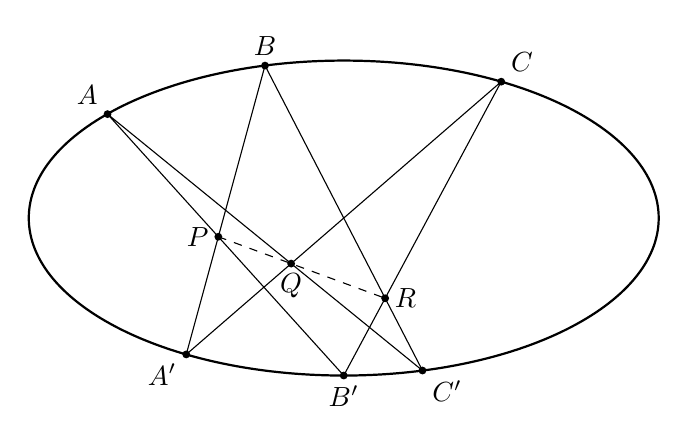
\begin{tikzpicture}[scale=2]

% Conic (ellipse for illustration)
\draw[thick] (0,0) ellipse (2 and 1);

% Points on the conic
\coordinate (A) at (-1.5,0.66);
\coordinate (B) at (-0.5,0.9682);
\coordinate (C) at (1,0.866);
\coordinate (Ap) at (-1,-0.866);
\coordinate (Bp) at (0,-1);
\coordinate (Cp) at (0.5,-0.9682);

% % Opposite sides intersections
\coordinate (P) at (-0.7963,-0.1187);
\coordinate (Q) at (-0.334,-0.2892);
\coordinate (R) at (0.263, -0.5093);

\draw[] (A)--(Bp) (A)--(Cp);
\draw[] (B)--(Ap) (B)--(Cp);
\draw[] (C)--(Ap) (C)--(Bp);

% % Pascal line
\draw[dashed] (P)--(R);

% % Labels
\node[above left] at (A) {$A$};
\node[circle, fill, inner sep=1pt] at (A) {};
\node[above] at (B) {$B$};
\node[circle, fill, inner sep=1pt] at (B) {};
\node[above right] at (C) {$C$};
\node[circle, fill, inner sep=1pt] at (C) {};
\node[below left] at (Ap) {$A'$};
\node[circle, fill, inner sep=1pt] at (Ap) {};
\node[below] at (Bp) {$B'$};
\node[circle, fill, inner sep=1pt] at (Bp) {};
\node[below right] at (Cp) {$C'$};
\node[circle, fill, inner sep=1pt] at (Cp) {};
\node[left] at (P) {$P$};
\node[circle, fill, inner sep=1pt] at (P) {};
\node[below] at (Q) {$Q$};
\node[circle, fill, inner sep=1pt] at (Q) {};
\node[right] at (R) {$R$};
\node[circle, fill, inner sep=1pt] at (R) {};

% \node[red] at (P) {$P$};
% \node[red] at (Q) {$Q$};
% \node[red] at (R) {$R$};

\end{tikzpicture} \]

\item Generalize (4.5) as follows: given 13 points $P_1, \dots, P_{13}$ in the plane, there are three additional deterined points $P_{14}, P_{15}, P_{16}$, such that all quartic curves through $P_1, \dots, P_{13}$ also pass through $P_{14}, P_{15}, P_{16}$.
What hypotheses are necessary on $P_1, \dots, P_{13}$ for this to be true.

\item If $D$ is any divisor of degree $d$ on the cubic surface (4.7.3), show that
\begin{equation*}
    p_a(D) \leq \begin{cases*}
        \cfrac{1}{6}(d - 1)(d - 2) & \text{if $d \equiv 1, 2 \mod{3}$}  \\
        \cfrac{1}{6}(d - 1)(d - 2) + \cfrac{2}{3} & \text{if $d \equiv 0 \mod{3}$.}
    \end{cases*}
\end{equation*}
Show furthermore that for every $d > 0$, this maximum is achieved by some irreducible nonsingular curve.

\item Show that a divisor class $D$ on the cubic surface contains an irreducible curve $\iff$ it contains an irreducible nonsingular curve $\iff$ it is either (a) one of the 27 lines, or (b) a conic (meaning a curve of degree 2) with $D^2 = 0$, or (c) $D.L \geq 0$ for every line $L$, and $D^2 > 0$.

\item If $C$ is an irreducible non-singular curve of degree $d$ on the cubic surface, and if the genus $g > 0$, then
\begin{equation*}
    g \geq \begin{cases*}
        \cfrac{1}{2}(d - 6) & \text{if $d$ is even, $d \geq 8$,} \\
        \cfrac{1}{2}(d - 5) & \text{if $d$ is odd, $d \geq 13$,}
    \end{cases*}
\end{equation*}
and this minimum value of $g > 0$ is achieved for each $d$ in the range given.

\item A curious consequence of the implications (iv) $\implies$ (iii) of (4.11) is the following numerical fact: Given integers $a, b_1, \dots, b_6$ such that $b_i > 0$ for each $i$, $a - b_i - b_j > 0$ for each $i, j$, and $2a - \sum_{i \neq j} b_i > 0$ for each $j$, we must necessarily have $a^2 - \sum b_i^2 > 0$.
Prove this directly (for $a, b_1, \dots, b_6 \in \R$) using methods of freshman calculus.

\item \textit{The Weyl Groups.} Given any diagram consisting of points and line segments joining some of them, we define an abstract group, given by the generators and relations, as follows: each point represents a generator $x_i$.
The relations are $x_i^2 = 1$ for each $i$; $(x_ix_j)^2 = 1$ if $i$ and $j$ are not joined by a line segment, and $(x_ix_j)^3 = 1$ if $i$ and $j$ are joined by a line segment.
\begin{itemize}
    \item[(a)] The \textit{Weyl group} $\A_n$ is defined using the diagram
    \tble{A/{}}
    of $n - 1$ points, each joined to the next.
    Show that it is isomorphic to the symmetric group $\Sigma_n$ as follows: map the generators of $\A_n$ to the elements $(12), (23), \dots, (n - 1, n)$ of $\Sigma_n$, to get a surjective homomorphism $\A_n \to \Sigma_n$.
    Then estimate the number of elements of $\A_n$ to show in fact it is an isomorphism.
    \item[(b)] The \textit{Weyl group} $\mathbf{E}_6$ is defined using the diagram
    \tble{E/{6}}
    Call the generators $x_1, \dots, x_5$ and $y$.
    Show that one obtains a surjective homomorphism $\mathbf{E}_6 \to G$, the group of automorphisms of the configuration of 27 lines (4.10.1), by sending $x_1, \dots, x_5$ to the permutations $(12), (23), \dots, (56)$ of the $E_i$, respectively, and $y$ to the element associated with the quadratic transformation based at $P_1, P_2, P_3$.
    \item[(c)] Estimate the number of elements in $\mathbf{E}_6$, and thus conclude that $\mathbf{E}_6 \cong G$.
\end{itemize}

\item Use (4.11) to show that if $D$ is any ample divisor on the cubic surface $X$, then $\cH^1(X, \fO_X(-D)) = 0$.
This is Kodaira's vanishing theorem for the cubic surface (III, 7.15).

\item Let $X$ be the Del Pezzo surface of degree 4 in $\P^4$ obtained by blowing up 5 points of $\P^2$ (4.7).
\begin{itemize}
    \item[(a)] Show that $X$ contains 16 lines.
    \item[(b)] Show that $X$ is a complete intersection of two quadric hypersurfaces in $\P^4$ (the converse follows from (4.7.1)).
\end{itemize}

\item Using the method of (4.13.1), verify that there are nonsingular curves in $\P^3$ with $d = 8$, $g = 6, 7$; $d = 9$, $g = 7, 8, 9$; $d = 10$, $g = 8, 9, 10, 11$.
Combining with (IV, \SS 6), this completes the determination of all possible $g$ for curves of degree $d \geq 10$ in $\P^3$.

\item Let $P_1, \dots, P_4$ be a fintie set of (ordinary) points of $\P^2$, no 3 collinear.
We define an \textit{admissible transformation} to be a quadratic transformation (4.2.3) centered at some three of the $P_i$ (call them $P_1, P_2, P_3$).
This gives a new $\P^2$, and a new set of $r$ points, namely $Q_1, Q_2, Q_3$, and the images of $P_4, \dots, P_r$.
We say that $P_1, \dots, P_r$ are in \textit{general position} if no three are collinear, and furthermore after any finite sequence of admissible transformations, the new set of $r$ points also have no three collinear.
\begin{itemize}
    \item[(a)] A set of 6 points is in general position if and only if no three are collinear and not all six lie on a conic.
    \item[(b)] If $P_1, \dots, P_r$ are in general position, then the $r$ points obtained by any finite sequence of admissible transformations are also in general position.
    \item[(c)] Assume the ground field $k$ is uncountable.
    Then given $P_1, \dots, P_r$ in general position, there is a dense $V \subseteq \P^2$ such that for any $P_{r + 1} \in V$, $P_1, \dots, P_{r + 1}$ will be in general position.
    \item[(d)] Now take $P_1, \dots, P_r \in \P^2$ in general position, and let $X$ be the surface obtained by blowing up $P_1, \dots, P_r$.
    If $r = 7$, show that $X$ has exactly 56 irreducible nonsingular curves $C$ with $g = 0$, $C^2 = -1$, and that these are the only irreducible curves with negative self-intersection.
    Ditto for $r = 8$, the number being 240.
    \item[(e)] For $r = 9$, show that the surface $X$ defined in (d) has infinitely many irreducible nonsingular curves $C$ with $g = 0$ and $C^2 = -1$.
\end{itemize}

\item For the \textit{Fermat cubic surface.} $x_0^3 + x_1^3 + x_2^3 + x_3^3 = 0$, find the equations of the 27 lines explicitly, and verify their incidence relations.
What is the group of automorphisms of this surface.

\end{enumerate}

\end{document}
